RFID systems that operating at the High Frequency (HF) band or lower use near-field based RFID design. The overall RFID system is electrically small that RFID reader antenna's load can be modulated. This is accomplished via near-field coupling between reader and tag and can be described in terms of Faraday's principle of magnetic induction. The reader tag has a alternating current pass through the coiled antenna that generates a magnetic field. When the RFID tag is within the reader's magnetic fields, resulting in an induced current within the RFID tag. This induced current yields a voltage across the tag, the tag has a minimal voltage requirement to turn it on. Once the tag turns on, it will generate its own magnetic fields to send data back to the RFID reader. The tag's load is applied to the reader's coiled antenna over time, causing a modulation. The RFID reader can encode this modulation into data.   

\begin{figure}[htp]
    \centering
    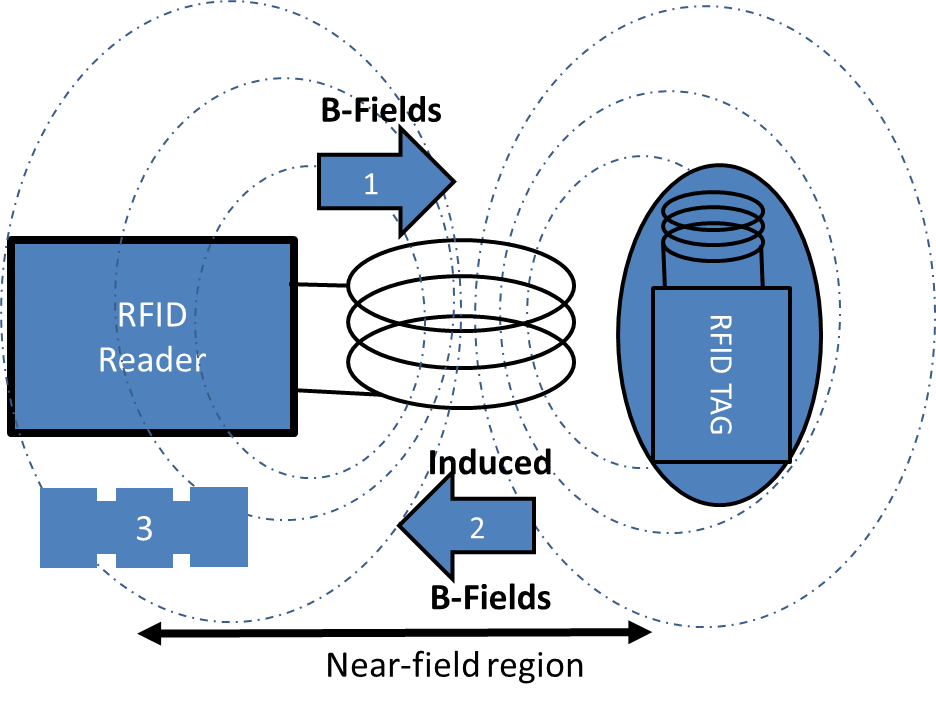
\includegraphics[scale=0.6]{Figs/nearField.png}
    \caption{Near-field power/communication set up RFID system. 1) RFID Reader creates B-Fields. 2) Reader B-Fields turns on tag, tag generates its own B-Field. 3) Tag's B-Field scatters into RFID Reader, encodes the modulation into data.}
    \label{fig:RFIDBlocks}
\end{figure}


%As previously mentioned the tag transmits its data via modulation. The two modulations are load modulation or modulated back-scatter. The load modulation uses the near-field coupling between reader and tag, can be describe via Faraday's principle. An alternating current is passed through the reader's (coiled) antenna, generating a magnetic field. Once the RFID tag is placed within the reader's fields this will result in an induced alternating voltage across the tag. This voltage will be used within the tag to turn its chip. Once the chip has been successfully activated, the tag yields its own magnetic fields that interact with the reader. The tag's load is applied to the reader's coiled antenna over time, causing a modulation. Typically load modulations operating under 100MHz (LF and HF).

